\section{Results}
\label{sec:testing} 

In this section, we present the findings of our evaluation. All test cases were repeated
ten times and the depicted values are trimmed averages taken after discarding the highest
and lowest values. Furthermore, graphs contain error bars, which extend from the $20^{th}$ to $80^{th}$ percentile unless explicitly indicated otherwise. Note that due to the random nature of losses in the network emulated during testing, outliers are inevitable, which is why we have chosen to focus on the middle population of the values. To the best of our knowledge, this approach does not produce any bias towards either protocol. 
% FIXME: why this, rather than presenting error bars? [csp] - done 

\subsection{Stall Events}
\label{sec:testing-stall}

The single most impactful impairment for MPEG-DASH video user experience has been found to be
stall events \cite{hossfeld2011quantification}. A perfect adaptation algorithm would
eliminate stall events during video play-out by pre-buffering content and by adjusting the
download quality of the video to match the network performance. However, in reality, stall
events occur, due to imperfect estimates of network conditions.

As we might expect, TCP Hollywood offers most benefit in the presence of moderate losses and high
delay. Figure \ref{fig:stall_delay2} shows the effect of network latency on the total
stall duration experienced over standard TCP and TCP Hollywood when the line rate and loss
rate were kept constant at 5Mbps and 0.2\% respectively. At lower network latency, loss
recovery is quick and hence TCP Hollywood and standard TCP have similar performance.
However, for higher network latency, head-of-line blocking in standard TCP prevents data
that has already arrived from reaching the application. When the missing TCP segment does
arrive, the client can read a larger amount of data into its play-out buffer. On average,
no more than one or two TCP Hollywood messages are discarded at network latencies of 300ms and
350ms. The additional performance comes from the ability of the rate adaptation algorithm in 
our TCP Hollywood-based MPEG-DASH client to compute metrics and decide the quality of the 
next chunk before the delivery of the current chunk (see Section \ref{sec:transport}). 
This would mean that the client does not have to wait unnecessarily for the arrival of 
retransmissions before requesting the next chunk, helping to avoid stalls.

\begin{figure}
  \centering
  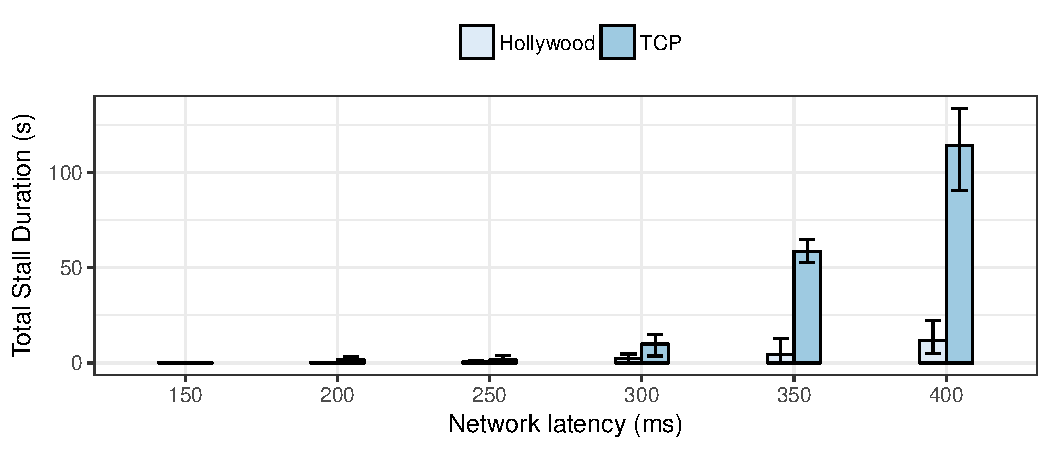
\includegraphics[width=\columnwidth]{figures/results/stall_sn_loss_p2.pdf}
  \caption{Stall events. Test networks were 5Mbps with 0.2\% loss with variable delay. The 
           client using standard TCP suffers more from stalls than the client using TCP Hollywood, 
           with the latter being able to minimise stalls in the presence of high network delay.}
  \label{fig:stall_delay2}
\end{figure}

\begin{figure}
  \centering
  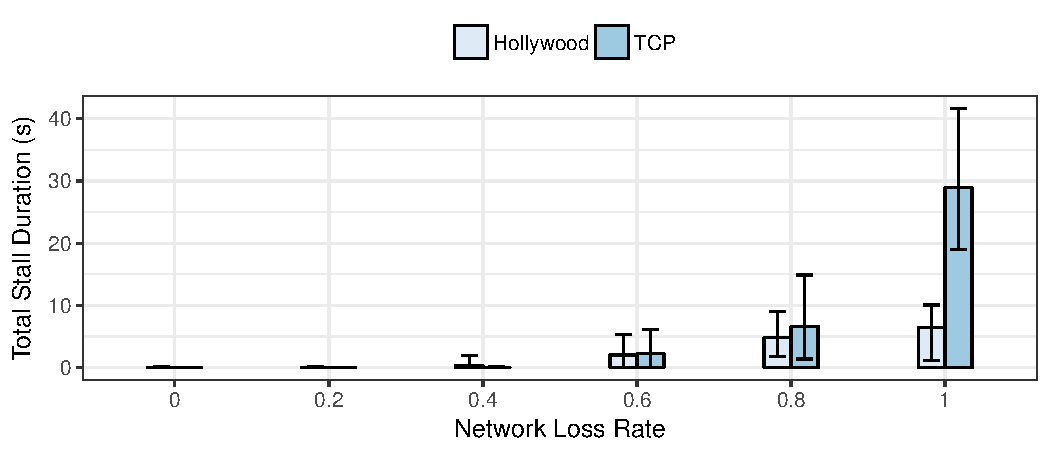
\includegraphics[width=\columnwidth]{figures/results/stall_sn_delay_d100.pdf}
  \caption{Stall events. Test networks were 5Mbps with 100ms delay and variable loss rates. With 
           high loss rates, loss recovery can be delayed due to lost retransmissions, leading 
           to more stall events for client using standard TCP.}
  \label{fig:stall_loss}
\end{figure}

When loss is high and delay is low, MPEG-DASH over TCP Hollywood and over standard TCP 
generally have similar performance. As packet loss increases, the TCP Hollywood-based 
client sees some performance benefit. Figure
\ref{fig:stall_loss} shows the results when network latency is 100ms, line rate is 5Mbps
and different network loss rates are used. When using loss rates of 0.6\% and 0.8\%, we
observed that the TCP Hollywood-based client is able to avoid some stall events by discarding 
some late arriving messages, however the benefit is very small in comparison to standard TCP 
as loss recovery is fast at low RTTs. At loss rates of 1\%, we observe that the advantage 
of using TCP Hollywood is significant, keeping the stall values for that client at around 5
seconds, in comparison with around 30 seconds in the case of the client using standard TCP 
for a 10 minute video. At high loss rates, the possibility of losing a retransmitted TCP 
segment become higher and loss recovery becomes a time consuming process even at lower 
network delays. 

\subsection{Start-up Delay}
We measure the start-up delay from the beginning of the test to the point when two seconds of
video (two chunks) have been downloaded and buffered, including the time taken to fetch the manifest
file. We use persistent connections for both standard TCP and TCP Hollywood, allowing the
TCP connection establishment and slow start latencies to be amortised across a longer
duration. In the case of TCP Hollywood, play-out can begin before the download of the
second chunk is complete, unlike standard TCP. However, as we use a receive ratio of 0.9,
the advantage is not significant for high speed networks. We still observe faster startup
values for TCP Hollywood in all scenarios because of its ability to request chunks
earlier. The higher the network latency, the greater the benefit of TCP Hollywood.

Figures \ref{fig:startup_delay2} and \ref{fig:startup_loss} show startup delay values
observed in our experiments. In the presence of higher losses, the startup delay can
become less stable and statistical significance in average values is lowered. For this
reason, the median value after eliminating the highest and the lowest observed values are
shown in the graphs.

\begin{figure}
  \centering
  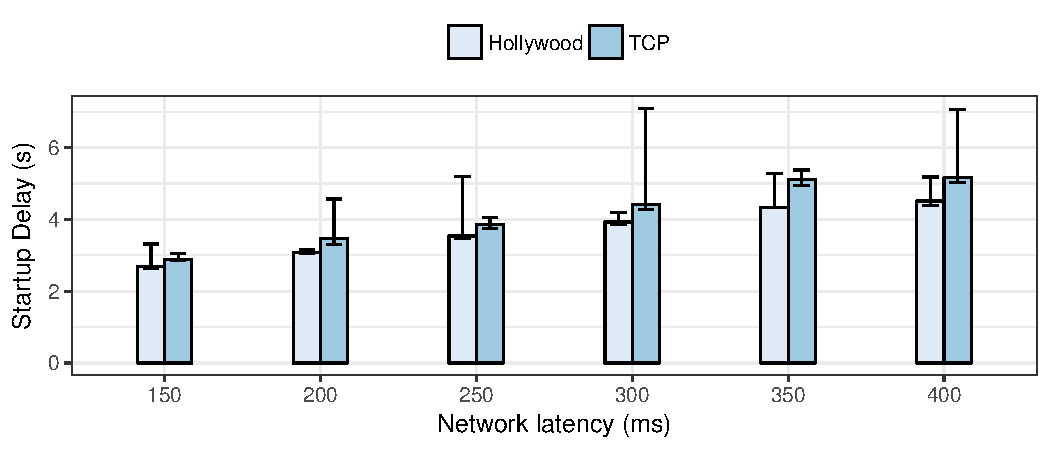
\includegraphics[width=\columnwidth]{figures/results/startup_sn_loss_p2.pdf}
  \caption{Start-up delay. Test networks were 5Mbps with 0.2\% loss with variable delay. 
           The higher the network latency, the greater the benefit of TCP Hollywood. }
  \label{fig:startup_delay2}
\end{figure}


\begin{figure}
  \centering
  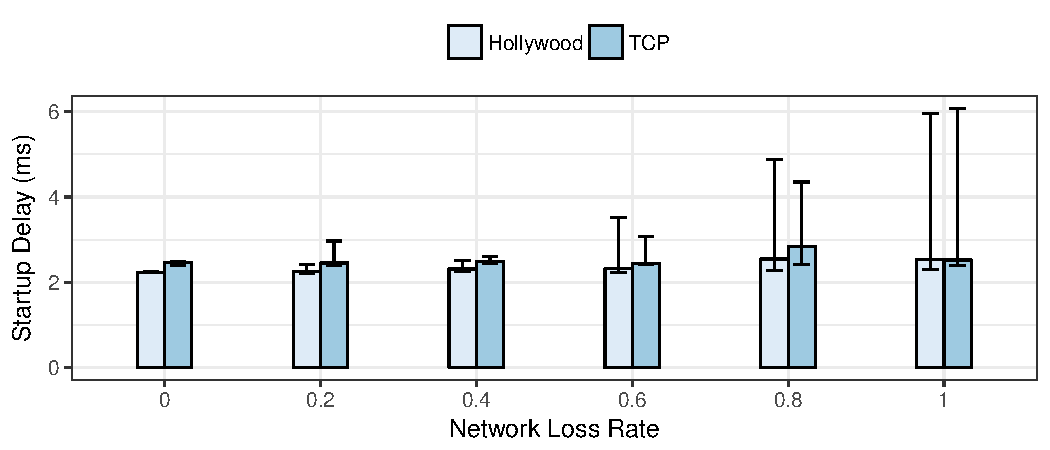
\includegraphics[width=\columnwidth]{figures/results/startup_sn_delay_d100.pdf}
  \caption{Start-up delay. Test networks were 5Mbps with 100ms with variable loss rates.  
           The start-up delay is slightly lower for the TCP Hollywood-based client, however, randomness of 
           emulated losses makes the values unpredictable. }
  \label{fig:startup_loss}
\end{figure}

\subsection{Adaptation and Stability}
While stall durations can be significantly reduced for high delay and high loss networks
by eliminating head-of-line blocking using TCP Hollywood, these improvements only hold
real significance if a TCP Hollywood-based client is able to deliver them while maintaining
the same level of video quality as a standard TCP-based client. Figure \ref{fig:rate_delay2} 
shows the effect of network latency on the average bit-rate of the video chunks for each transport
protocol. The error bars indicate the standard deviation in the downloaded chunk bit-rate; a higher standard deviation indicates a higher range of bit-rate switching. It can be seen that TCP Hollywood has a higher average bit-rate with a similar
level of standard deviation when network delay is 150ms and 200ms. For higher network
delay, TCP Hollywood continues to deliver chunks at a similar average bit-rate value than
standard TCP. In general, standard TCP appears to be more stable, as exhibited by the
percentage of chunks with a rate drop shown in Figure \ref{fig:ratechange_delay2}. A rate
drop is counted each time a chunk is downloaded at a bit-rate which is lower than the chunk
immediately before it. The difference in rate drops is equivalent to about 1 additional
drop observed per minute for TCP Hollywood than for standard TCP. We show only the rate drops here as they have a higher impact on user experience than upward switching, however, the observed trends were similar for both. 

\begin{figure}
  \centering
  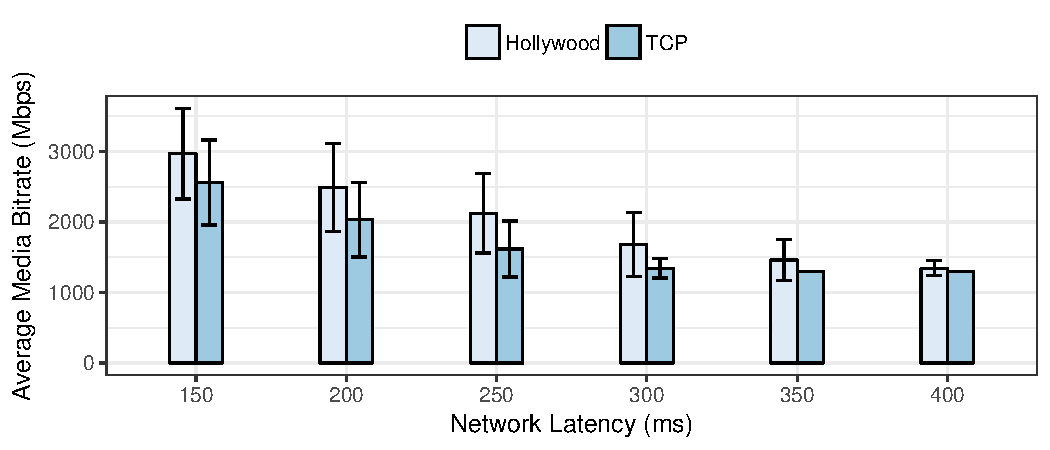
\includegraphics[width=\columnwidth]{figures/results/bitrate_sn_loss_p2.pdf}
  \caption{Adaptation and stability. Test networks were 5Mbps with 0.2\% loss with variable 
           delay. The error bars represent standard deviation, indicating bit-rate switching. For higher delay values, 
           standard TCP shows lower standard deviation because it remains mostly at the 
           lowest available bit-rate. }
  \label{fig:rate_delay2}
\end{figure}

\begin{figure}
  \centering
  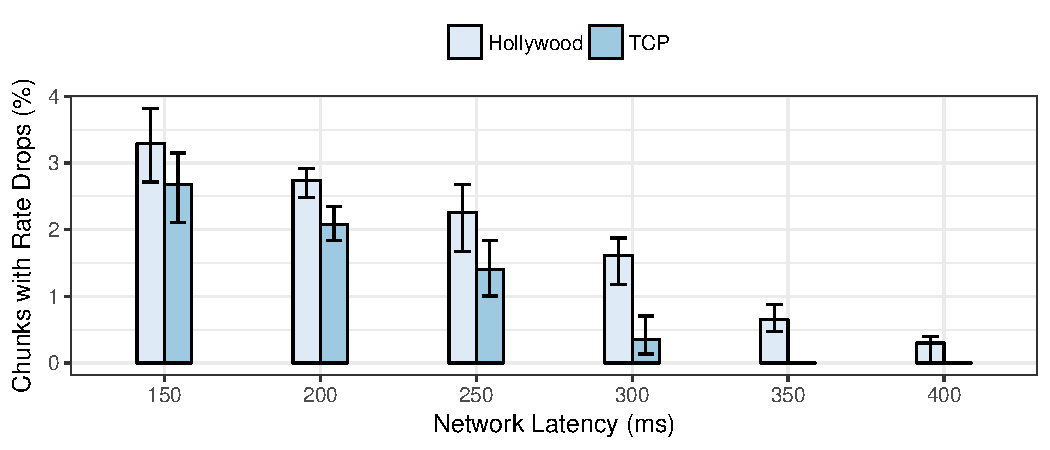
\includegraphics[width=\columnwidth]{figures/results/ratedrops_sn_loss_p2.pdf}
  \caption{Adaptation and stability. Test networks were 5Mbps with 0.2\% loss with variable 
           delay. The graph shows the percentage of chunks that were downloaded at a lower 
           rate than the previous one. The standard TCP adaptation algorithm is more stable 
           for all networks. The test video had 597 chunks.}
  \label{fig:ratechange_delay2}
\end{figure}

We observe that when packet loss is kept under 0.1\%, clients using both standard TCP and TCP 
Hollywood exhibit similar behaviour. As shown in Figure \ref{fig:rate_loss}, where network delay is 100ms, 
the TCP Hollywood-based client was able to deliver a higher average bit-rate than the standard TCP-based client, as
loss rates increased. Figure \ref{fig:ratechange_loss} shows the stability of the rate adaptation
algorithm under both standard TCP and TCP Hollywood. At a loss rate of 0.2\%, we found that the
TCP Hollywood-based client had higher stability than the standard TCP-based client. However,
for higher loss rate values, the TCP Hollywood-based client is less stable, as it attempts
to download higher bit-rate chunks, while the standard TCP-based client maintains stability
at the lowest bit-rate.

\begin{figure}
  \centering
  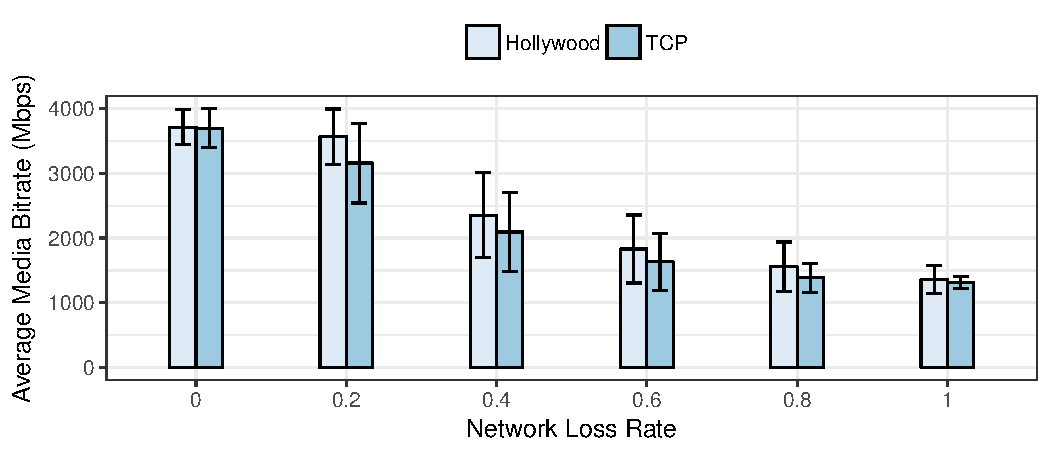
\includegraphics[width=\columnwidth]{figures/results/bitrate_sn_delay_d100.pdf}
  \caption{Test networks were 5Mbps with 100ms with variable loss rates. TCP Hollywood 
           significantly outperforms standard TCP at loss rate of 0.2\% with a higher 
           average rate and lower standard deviation. Error bars represent standard deviation.}
  \label{fig:rate_loss}
\end{figure}

\begin{figure}
  \centering
  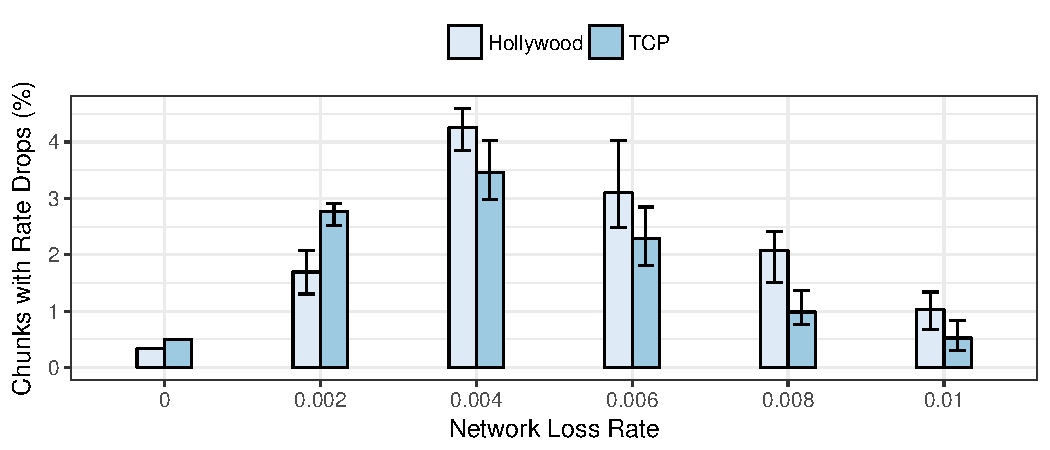
\includegraphics[width=\columnwidth]{figures/results/ratedrops_sn_delay_d100.pdf}
  \caption{Test networks were 5Mbps with 100ms with variable loss rates. Hollywood is more 
           stable for 0.2\% and no loss cases, however, at higher loss levels, standard TCP 
           becomes more stable.}
  \label{fig:ratechange_loss}
\end{figure}

\subsection{Quality of Experience}
None of the previously discussed metrics quantify the impact of the dropped messages
on a TCP Hollywood-based DASH client. A discarded message will result in visual impairments
that are not possible for a client using a reliable TCP stream. Figure \ref{fig:qoe_delay2} 
and \ref{fig:qoe_loss} show the observed PSNR and SSIM values of the received streams for the 
different transport options. The figures show box plots of frame-level PSNR and SSIM values 
observed during multiple
iterations of the test. Note that although the two objective QoE metrics represent the
quality of the chunks and the level of visual impairments due to discarded packets, it
does not show the impact of stall events, which were discussed in
Section \ref{sec:testing-stall}. Across all of the tests we ran in these experiments,
about 30\% of streams discarded at least one message during the 10 minutes of the video,
however, of these only 5\% lost more than 10 messages. Furthermore, the impact of a lost
message is most evident when a part of an I frame is lost. However, since chunks begin with
an I frame, the effect of even the worst visual impairment does not propagate farther than
the duration of the chunk, which in our case is 1 second.

\begin{figure}
  \centering
  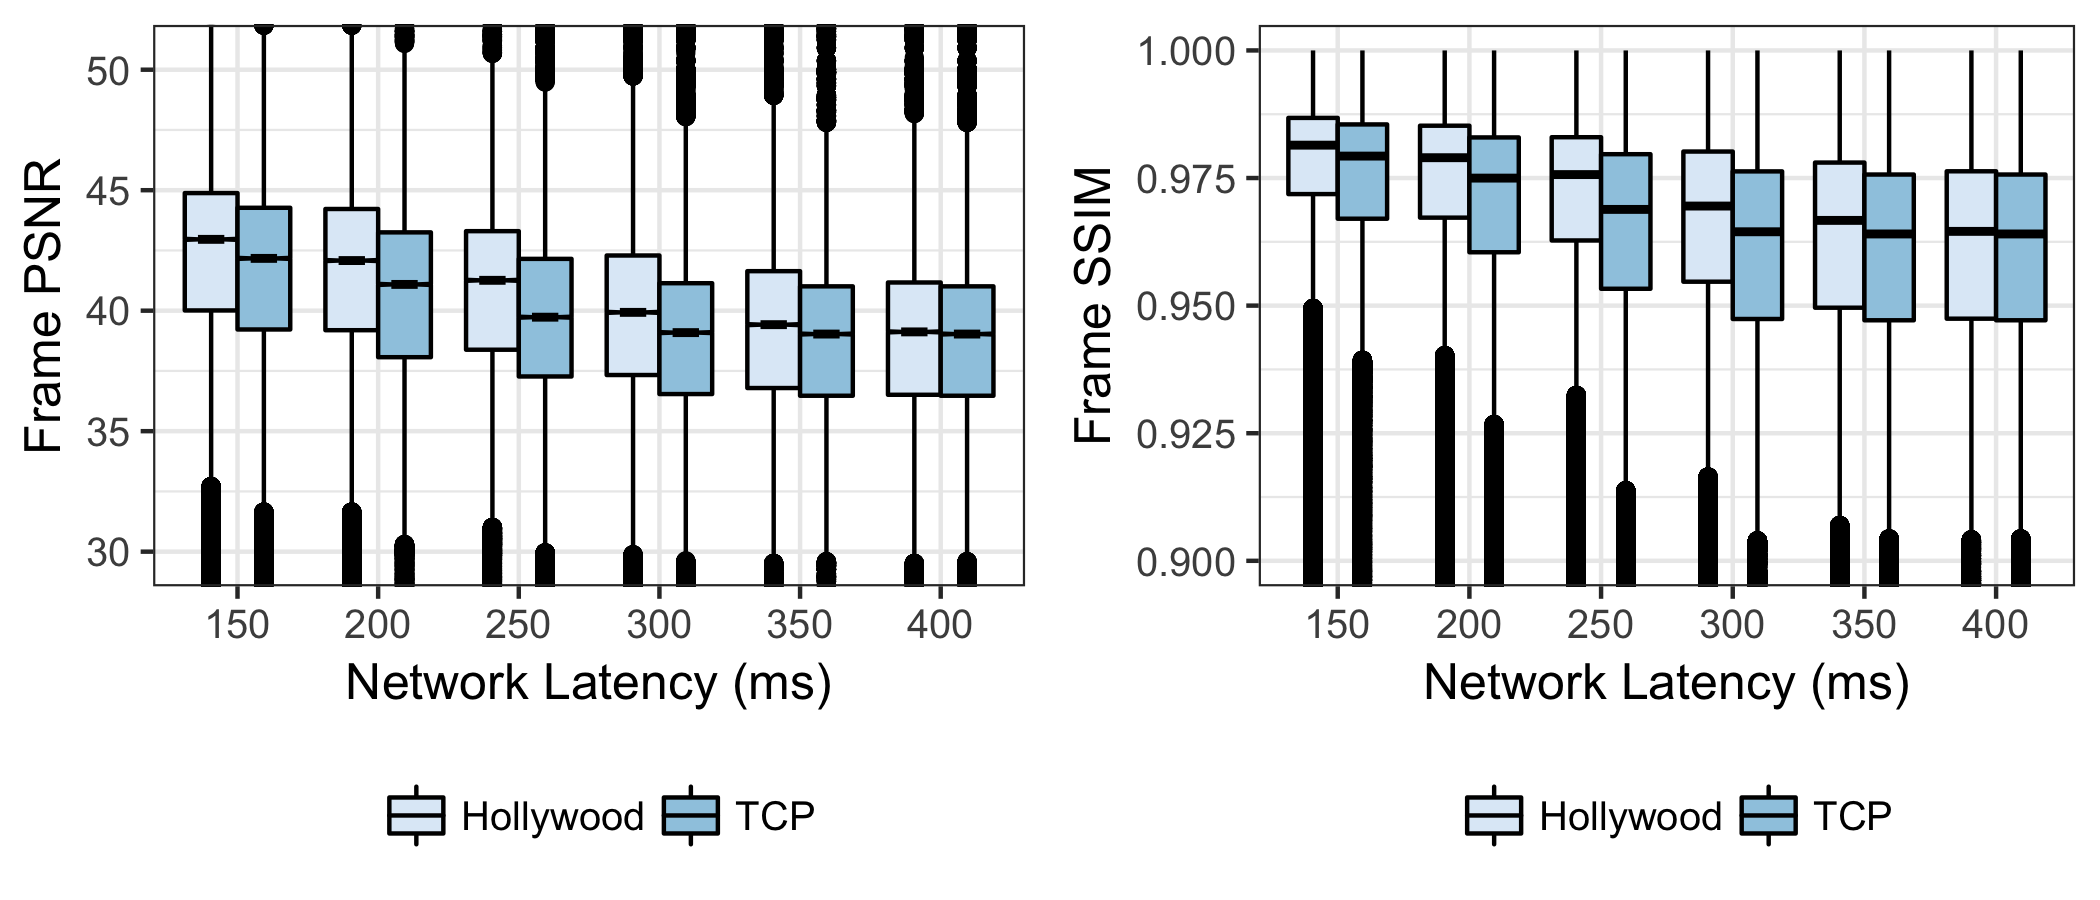
\includegraphics[width=\columnwidth]{figures/results/qoe_sn_loss_p2.png}
  \caption{Impact of delay on quality of experience. Test networks were 5Mbps with 0.2\%loss 
           with variable delay.}
  \label{fig:qoe_delay2}
\end{figure}

\begin{figure}
  \centering
  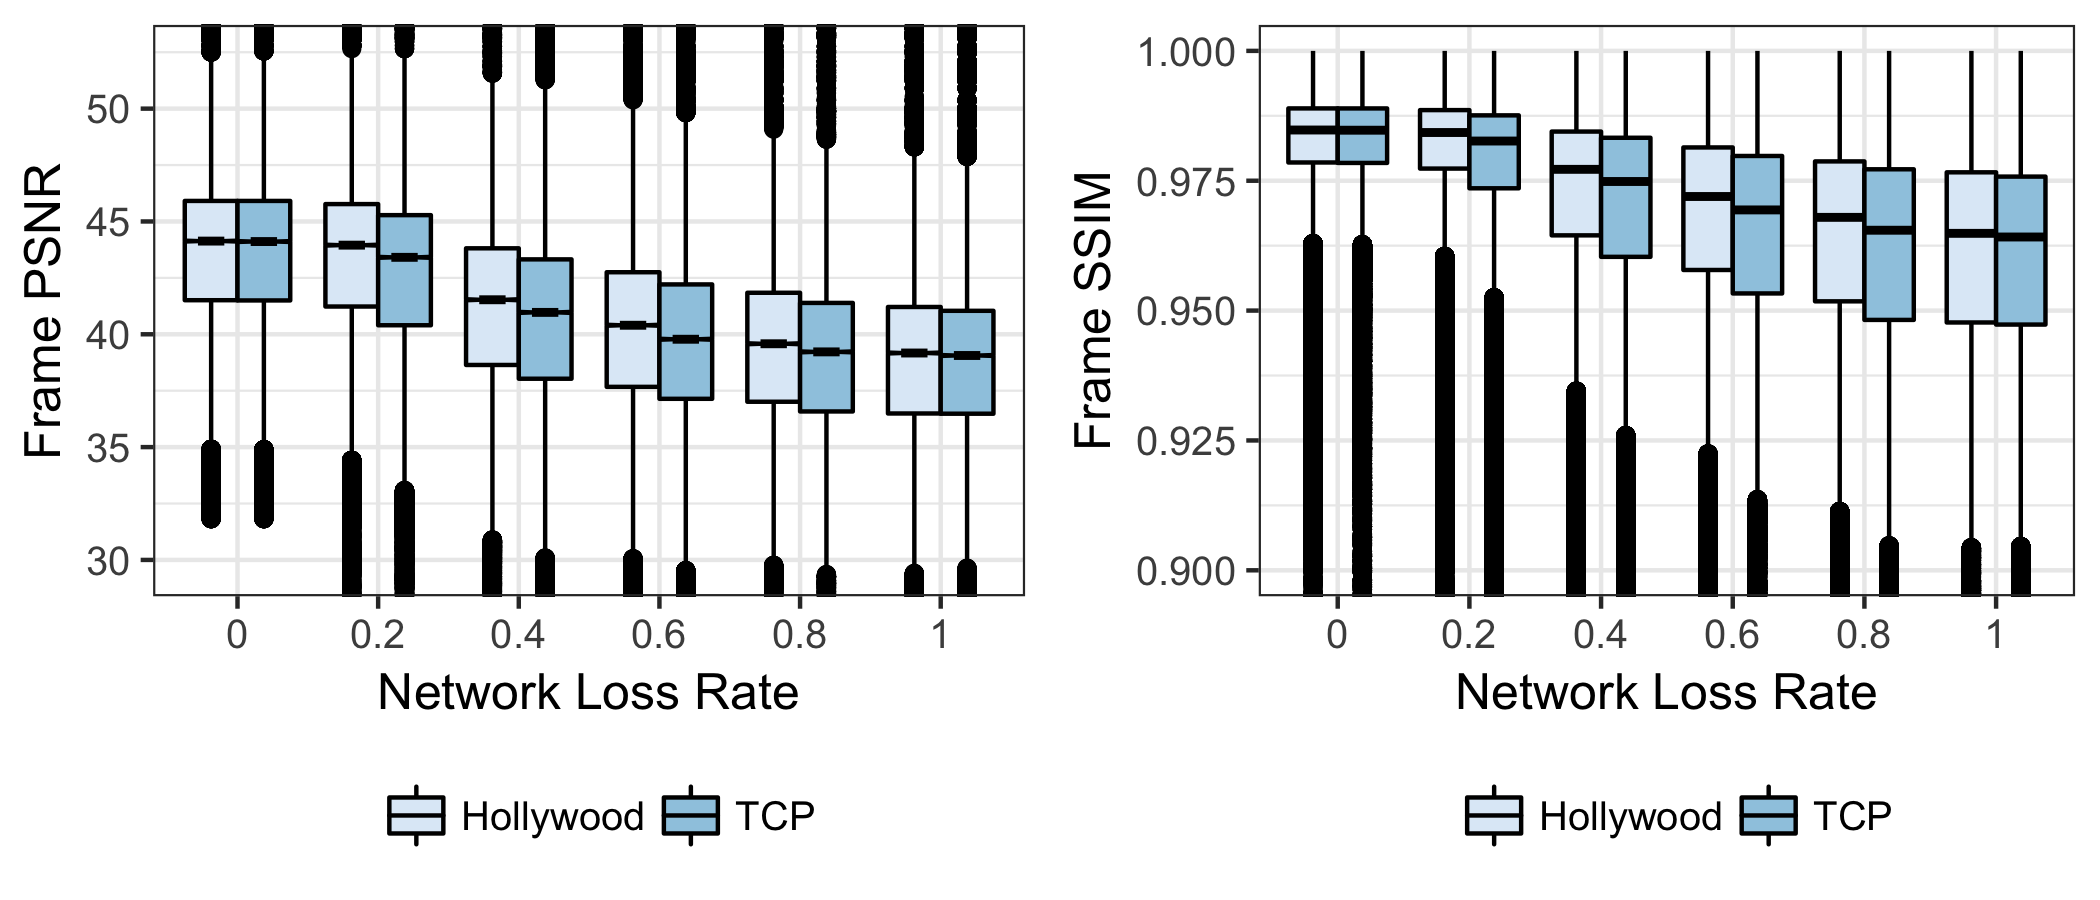
\includegraphics[width=\columnwidth]{figures/results/qoe_sn_delay_d100.png}
  \caption{Impact of packet loss on quality of experience. Test networks were 5Mbps with 100ms 
           with variable loss rates.  The TCP Hollywood-based client maintains a higher PSNR 
           and SSIM than standard TCP.}
  \label{fig:qoe_loss}
\end{figure}

\subsection{Other Testing}
\label{sec:other_testing}

We represent in this paper results from cases where the stall events were within
acceptable limits for a range of latency and loss values. However, we tested for other
conditions as well. For delay variation testing with a fixed loss rate at 0.03\%, we found
that both protocols performed equally with no stall event for delays as high as 400ms. For
a loss rate of 0.8\%, the stall duration was about 300s even at a delay of 200ms for the
standard TCP-based client. For the TCP Hollywood-based client, the stall events were reduced 
by 40\% but nearly 150
messages were discarded. Similarly, for a loss rate of 2\%, stall durations were as high as
300s when running over standard TCP with a 100ms network latency, while the use of 
TCP Hollywood reducing stall durations 
to around 230s at the cost of heavy losses. Given that such high levels of stalling will
any way be unacceptable to users, we feel that attempting to evaluate which protocol
performed better is of little consequence.

To evaluate the suitability of the adaptation algorithm in fluctuating network conditions,
we ran tests using the twelve network profiles (\emph{a} - \emph{l}) used by Spiteri et.
al.\ in their evaluation of the BOLA algorithm \cite{spiteri2016bola}. The profiles cover a
wide range of loss rates, delays and bandwidths and network conditions are changed during
the tests every 30 seconds. Since some bandwidths in the test were lower than the lowest
bit-rate in our test videos and the buffer length was limited to 16 seconds, we observed
stall events, especially for the more aggressively changing profiles (profiles \emph{g} to
\emph{l}). Generally, the use of TCP Hollywood lowered the stall events, as shown in Figure
\ref{fig:stall_profiles}. Start-up delay was similar for clients using both protocols,
although some profiles with longer network delays in the beginning benefited from the use of TCP Hollywood as shown in Figure \ref{fig:startup_profiles}.

\begin{figure}
  \centering
  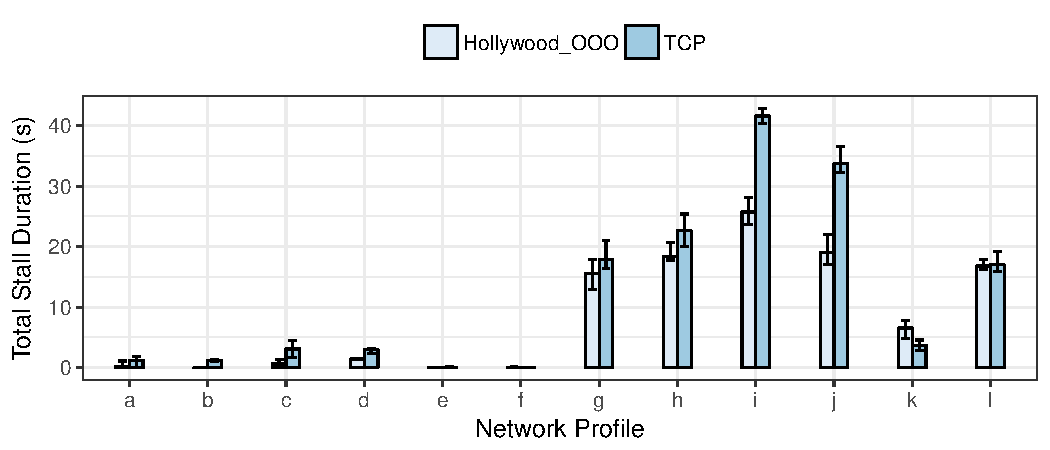
\includegraphics[width=\columnwidth]{figures/results/stall_vn_all.pdf}
  \caption{Stall events are reduced for TCP Hollywood for all except profile k, where 
           latencies are under 20 ms and bandwidth levels between 9Mbps and 1Mbps. }
  \label{fig:stall_profiles}
\end{figure}

\begin{figure}
  \centering
  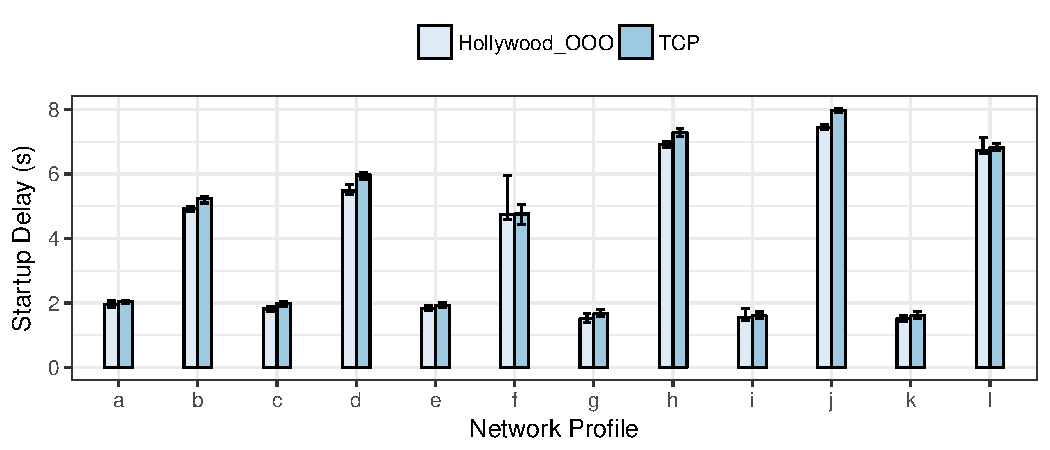
\includegraphics[width=\columnwidth]{figures/results/startup_vn_all.pdf}
  \caption{Startup delays observed for different network profiles. }
  \label{fig:startup_profiles}
\end{figure}




\begin{figure}
  \centering
  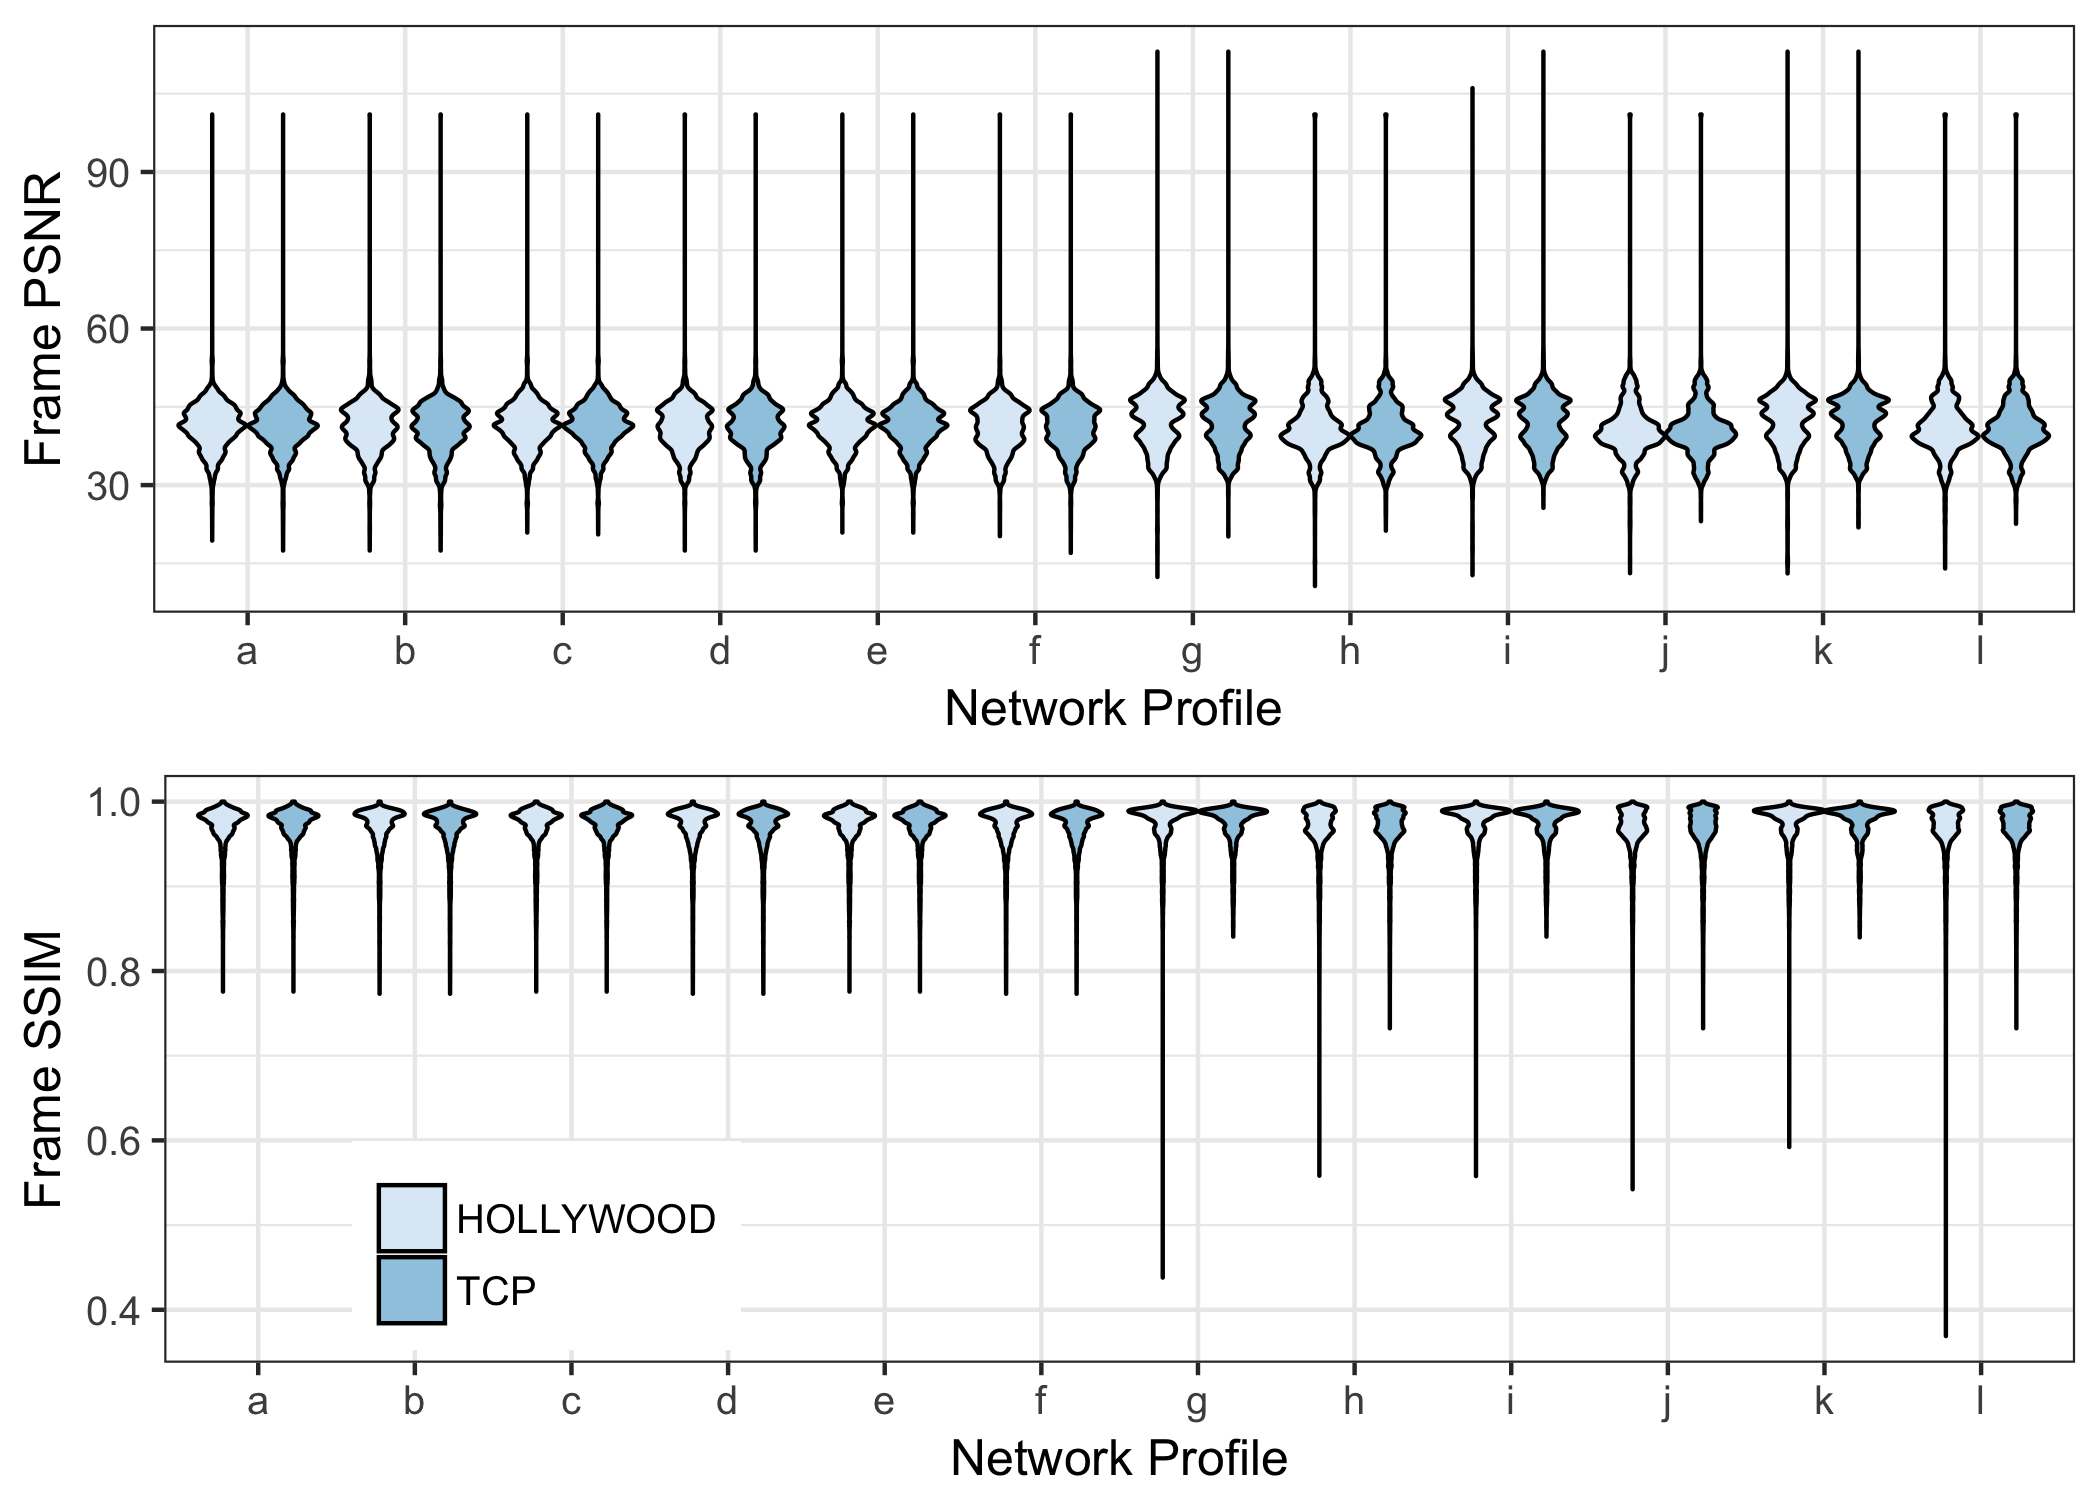
\includegraphics[width=\columnwidth]{figures/results/qoe_vn_all.png}
  \caption{Quality of experience profiles. PSNR and SSIM values of various network profiles 
           revealed similar results for both standard TCP and TCP Hollywood-based clients. The 
           shape of the violin graph reveals more information about the frequency of values, 
           showing the similarity in the download quality of both protocols with the tails in 
           SSIM plot representing the effect of lost messages.}
  \label{fig:qoe_profiles}
\end{figure}

A violin plot of the PSNR and SSIM values shows the frequency of each value in Figure 
\ref{fig:qoe_profiles}. The similarity in the shape of the plot for clients using both 
standard TCP and TCP Hollywood shows that both protocols downloaded similar quality chunks, 
as observed in the average bit-rate results shown in Figure \ref{fig:rate_profiles}. The TCP Hollywood-based client had 
a lower number of downward rate switches than the standard TCP-based client for almost all 
profiles, as shown in Figure \ref{fig:ratechange_profiles}. The client using BOLA working
with TCP Hollywood generally adapted faster to a higher bit-rate and was able to sustain a
higher bit-rate for longer than the client using standard TCP. However, this also meant that 
the TCP Hollywood client would drop suddenly to a lower rate while the standard TCP-based 
client would drop
gradually. If the degradation lasted less than the 30 seconds defined by the profiles, as
may be the case for real networks, the TCP Hollywood-based client is more likely to sustain 
the current bit-rate without dropping at all. A sample bit-rate adaptation for network profile 
\emph{g} is shown in Figure \ref{fig:adaptation_profile}. Note from Figure \ref{fig:qoe_profiles}
previously showed that the TCP Hollywood-based client does suffer from message losses in profile 
\emph{g} and future work should include exploring improvements in the adaptation algorithm to 
limit the number of discarded messages in favour of stalls in the presence of high losses. 

\begin{figure}
  \centering
  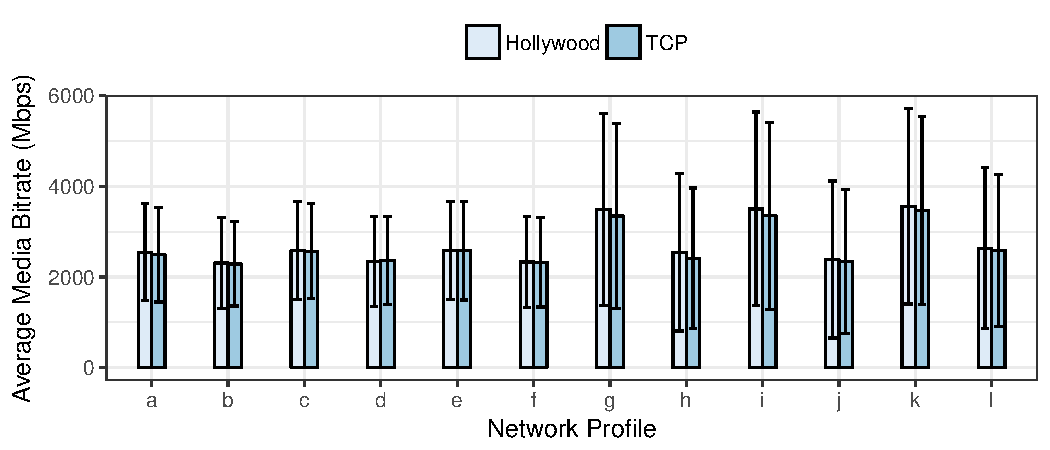
\includegraphics[width=\columnwidth]{figures/results/bitrate_vn_all.pdf}
  \caption{The average media bit rate was similar for all network profiles. The slight improvement for TCP Hollywood is further explained in Figure \ref{fig:adaptation_profile} }
  \label{fig:rate_profiles}
\end{figure}


\begin{figure}
  \centering
  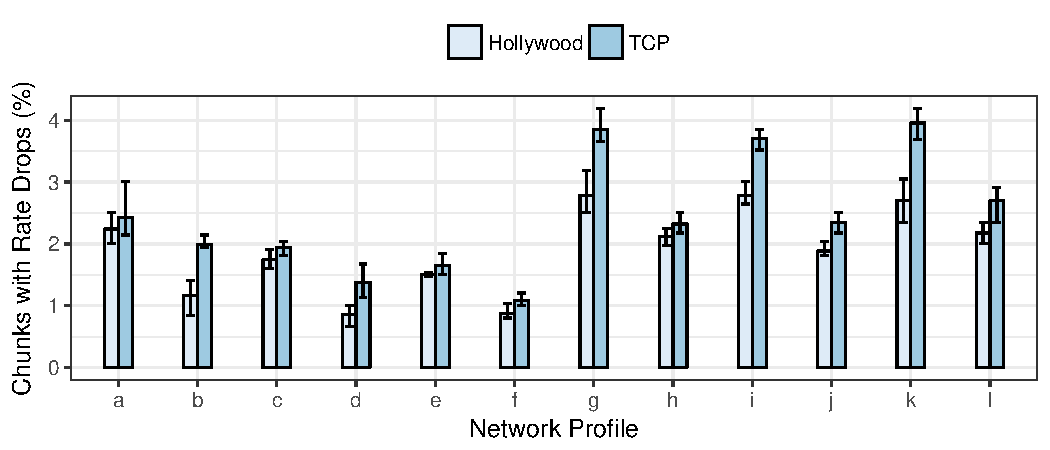
\includegraphics[width=\columnwidth]{figures/results/ratedrops_vn_all.pdf}
  \caption{Fewer rate drops were observed over TCP Hollywood for all network profiles.}
  \label{fig:ratechange_profiles}
\end{figure}

\begin{figure}
  \centering
  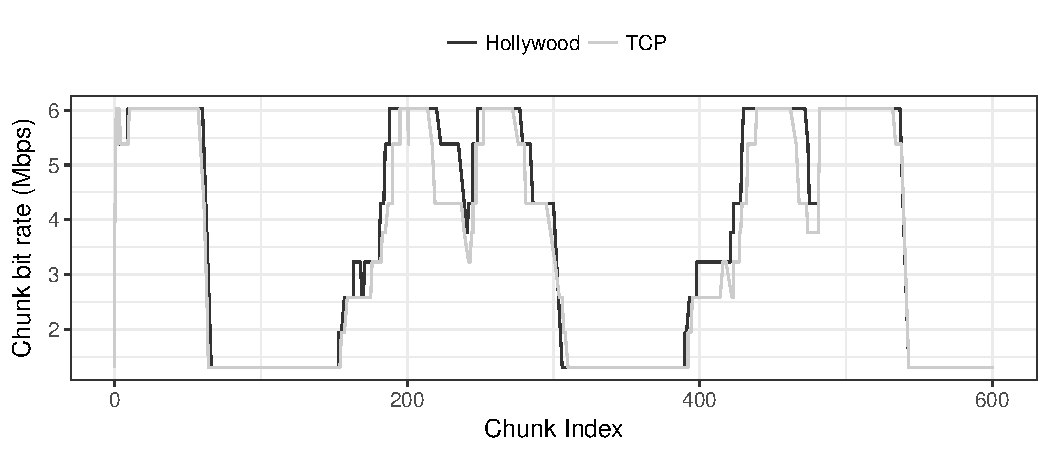
\includegraphics[width=\columnwidth]{figures/results/timeline_example_vn.pdf}
  \caption{TCP Hollywood allows the adaptation algorithm to adapt more quickly to higher bit-rates and also to sustain them for longer periods in the presence of network degradation. }
  \label{fig:adaptation_profile}
\end{figure}
